
\chapter{Week7}

\section{Tuesday}\index{week7_Tuesday_lecture}\subsection{Quadratic form}
The graphs of the following equations are easy to plot:
\begin{gather}
x^2+y^2=1\label{eq:17.1}\implies\text{ Circle}.\\
\frac{x^2}{2}+\frac{y^2}{5}=1\label{eq:17.2}\implies\text{ Elipse}.\\
\frac{x^2}{2}-\frac{y^2}{5}=1\label{eq:17.3}\implies\text{ Hyperbola}.\\
\left.\begin{aligned}
x^2&=\alpha y\\
y^2&=\alpha x
\end{aligned}\right\}\implies\text{ Parabola}.\label{eq:17.4}
\end{gather}
\begin{figure}[H]
\centering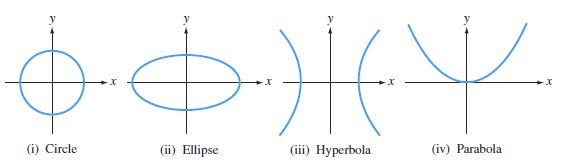
\includegraphics{week7/shape}
\caption{graph for quadratic form equations of two variables}
\end{figure}
The equations $(\ref{eq:17.1})-(\ref{eq:17.4})$ is the \textit{quadratic form equations of two variables}. Now we give the general form for quadratic equations:
\begin{definition}[Quadratic form]
The formula of \emph{quadratic form} is given by
\[
\bm x\trans\bm A\bm x
\]
where $\bm A\in\mathbb{S}^n$ and $\bm x\in\mathbb{R}^{n}$.

Moreover, sometimes we write $\bm x\trans\bm A\bm x$ as:
\[
\bm x\trans\bm A\bm x=\sum_{i,j=1}^{n}x_ix_ja_{ij}
\]
where $x_i$ is the $i$th entry of $\bm x$ and $a_{ij}$ are $(i,j)$th entry of $\bm A$.
\end{definition}
Moverover, we say an equation is the \emph{conic section of quadratic form} if it can be written as
\[
\bm x\trans\bm A\bm x=1.
\]

You may be confused why the quadratic form requires the symmetric constraint. Now we give the reason:
\begin{itemize}
\item
It is easy to verify $\bm x\trans\bm A\bm x=\bm x\trans\bm A\trans\bm x$.
\item
Hence given any matrix $\bm A$, we always have
\begin{align*}
\bm x\trans\left(\frac{\bm A+\bm A\trans}{2}\right)\bm x&=\frac{1}{2}\bm x\trans\bm A\bm x+\frac{1}{2}\bm x\trans\bm A\trans\bm x\\&=\frac{1}{2}\bm x\trans\bm A\bm x+\frac{1}{2}\bm x\trans\bm A\bm x\\&=\bm x\trans\bm A\bm x.
\end{align*}
\end{itemize}
Note that $\left(\frac{\bm A+\bm A\trans}{2}\right)$ is \textit{symmetric}! Hence given any $\bm A$, since $\bm x\trans\bm A\bm x=\bm x\trans\left(\frac{\bm A+\bm A\trans}{2}\right)\bm x$, it suffices to consider a symmetric matrix.
\begin{example}
Given the equation $3x^2+2xy+3y^2=1$, how we transform it into the conic section of quadratic form? How can we determine its shape in view of matirx?

Actually, It can be written as
\begin{equation}
\begin{pmatrix}
x&y
\end{pmatrix}\begin{pmatrix}
3&1\\1&3
\end{pmatrix}\begin{pmatrix}
x\\y
\end{pmatrix}=1.\qquad\qquad\text{\emph{conic section of quadratic form.}}
\label{conic_section}
\end{equation}

We could obatin a simpler version of the conic section of quadratic form, i.e., the middle matrix should be diagonal.
We define $\bm A=\begin{pmatrix}
3&1\\1&3
\end{pmatrix}.$  Since $\bm A\in\mathbb{S}^2$, it admits the eigenvalue decomposition:
\[
\bm A=\bm Q\Lambda\bm Q\trans
\]
where $\Lambda=\begin{pmatrix}
\lambda_1&\\&\lambda_2
\end{pmatrix}$, $\bm Q=\begin{bmatrix}
\bm x_1&\bm x_2
\end{bmatrix}$.

Thus we convert equation (\ref{conic_section}) into
\begin{equation}
\begin{pmatrix}
x&y
\end{pmatrix}\bm Q\Lambda\bm Q\trans\begin{pmatrix}
x\\y
\end{pmatrix}=1
\implies
\tilde{\bm x}\trans\Lambda\tilde{\bm x}=1.\label{Eq:8:6}
\end{equation}
where $\tilde{\bm x}=\bm Q\trans\begin{pmatrix}
x\\y
\end{pmatrix}=\begin{pmatrix}
\tilde x_1\\\tilde x_2
\end{pmatrix}$.\\
Then how to determine the shape of this equation? We just do matrix multiplication of Eq.(\ref{Eq:8:6}) to obtain:
\[
\lambda_1\tilde x_1^2+\lambda_2\tilde x_2^2=1.
\]
After computation, we find $\lambda_1,\lambda_2>0$. Hence this equation is an \emph{elipse.}
\end{example}
\subsection{Convex Optimization Preliminaries}
Now we recall how to compute derivative for matrix:
\[
\frac{\partial(f\trans g)}{\partial x}=\frac{\partial f(x)}{\partial x}g(x)+\frac{\partial g(x)}{\partial x}f(x)
\]
Examples of matrix derivatives:
\begin{align*}
\frac{\partial(a\trans \bm x)}{\partial \bm x}&=a
\\
\frac{\partial(a\trans \bm A\bm x)}{\partial \bm x}&=\frac{\partial((\bm A\trans a)\trans\bm x)}{\partial \bm x}=\bm A\trans a\\
\frac{\partial(\bm A\bm x)}{\partial \bm x}&=\bm A\trans\\
\frac{\partial(\bm x\trans\bm A\bm x)}{\partial \bm x}&=\bm A\bm x+\bm A\trans\bm x
\end{align*}
\begin{example}\qquad\\
Given $f(\bm x)=\frac{1}{2}\bm x\trans\bm A\bm x+\bm b\trans\bm x$. We want to do the optimization:
\[
\min_{\bm x\in\mathbb{R}^{n}}f(\bm x)
\]
How to find the optimal solution? The direct idea is to take the first order derivative:
\begin{align*}
\frac{\partial f}{\partial \bm x}&=\frac{1}{2}\frac{\partial(\bm x\trans\bm A\bm x)}{\partial \bm x}+\frac{\partial(\bm b\trans\bm x)}{\bm x}\\
&=\frac{1}{2}(\bm{Ax}+\bm A\trans\bm x)+\bm b.
\end{align*}
Since $\bm A$ is symmetric, we obtain
\[
\frac{\partial f}{\partial \bm x}=\bm{Ax}+\bm b.
\]
If $\bm x^{*}$ is an optimal solution, then it must satisfy:
\[
\nabla f(\bm x^{*})=\frac{\partial f(\bm x^{*})}{\partial \bm x}=\bm 0\implies
\bm A\bm x^{*}+\bm b=\bm 0.
\]
There may follow these cases:
\begin{itemize}
\item
If equation $\bm{Ax}+\bm b=\bm 0$ has no solution, then $f(\bm x)$ is unbounded. (We omit the proof of this statement)
\item
If equation $\bm{Ax}+\bm b=\bm 0$ has a solution $\bm x^{*}$, it doesn't mean $\bm x^{*}$ is an optimal solution. (Note that the reverse is true.)

Let's raise a counterexample: if we set
\[
\begin{array}{lll}
\bm A=\begin{bmatrix}
1&0\\0&-1
\end{bmatrix},
&
\bm b=\bm 0,
&
\bm x=\begin{pmatrix}
x_1\\x_2
\end{pmatrix},
\end{array}
\]
then $f(\bm x)=\frac{1}{2}(x_1^2-x_2^2)$. One solution to $\bm{Ax}+\bm b=\bm 0$ is $\bm x^*=\begin{pmatrix}
0\\0
\end{pmatrix}$. 

Obviously, $\bm x^{*}$ is not a optimal solution. If $x_1=0,x_2\rightarrow\infty$, then $f(\bm x)\rightarrow-\infty$!
\end{itemize}
\end{example}

\subsubsection{Second optimality condition}
If $\bm x^{*}$ is a optimal solution to $f(\bm x)$, what else condition should $\bm x^{*}$ satisfy?

Let's take $f(\bm x)=\frac{1}{2}\bm x\trans\bm A\bm x+\bm b\trans\bm x$ as an example, we want to find $\bm x^{*}$ s.t. 
\[
\min f(\bm x)=f(\bm x^{*}).
\]

Firstly, we write $f(\bm x)$ into its \textit{taylor expansion}:
\begin{equation}
f(\bm x)=f(\bm x^{*})+\inp{\nabla f(\bm x^*)}{\bm x-\bm x^*}+\frac{1}{2}(\bm x-\bm x^*)\trans\nabla^2f(\bm x^*)(\bm x-\bm x^*).\label{Eq:8:7}
\end{equation}

Note that $\nabla^2f(\bm x^*)$ is the Hessian matrix of $f(\bm x^*)$, which is defined as 
\[
\nabla^2f(\bm x^*):=\begin{bmatrix}
\frac{\partial^2 f(\bm x^*)}{\partial x_{i}\partial x_{j}}
\end{bmatrix}=\nabla(\nabla f(\bm x^*)).
\]

We compute $\bigtriangledown f(\bm x)$ and $\bigtriangledown^2 f(\bm x)$:
\begin{align*}
\bigtriangledown f(\bm x)&=\frac{1}{2}(\bm{Ax}+\bm A\trans\bm x)+\bm b.\\
\bigtriangledown^2 f(\bm x)&=\bigtriangledown\left[\frac{1}{2}(\bm{Ax}+\bm A\trans\bm x)+\bm b\right]=\frac{1}{2}\bigtriangledown(\bm{Ax})+\frac{1}{2}\bigtriangledown(\bm A\trans\bm x)
=\frac{1}{2}(\bm A+\bm A\trans).
\end{align*}

If assume $\bm A$ is \emph{symmetric}, then we have $\nabla f(\bm x)=\bm A\bm x+\bm b$ and $\nabla^2 f(\bm x)=\bm A$.

Since the optimal solution $\bm x^*$ satisfies $\bigtriangledown f(\bm x^*)=\bm 0$, we deive 
\[\inp{\bigtriangledown f(\bm x^*)}{\bm x-\bm x^*}=0.\]

 Then substituting it into Eq.(\ref{Eq:8:7}), we obtain:
\[
f(\bm x)=f(\bm x^{*})+\frac{1}{2}(\bm x-\bm x^*)\trans\bigtriangledown^2f(\bm x^*)(\bm x-\bm x^*).
\]

Or equivalently, $f(\bm x)-f(\bm x^{*})=\frac{1}{2}(\bm x-\bm x^*)\trans\bm A(\bm x-\bm x^*).$

Since $\bm x^*$ is optimal that minimize $f(\bm x)$, $LHS=f(\bm x)-f(\bm x^*)\ge0$ for $\forall\bm x$. It follows that
\[ 
\frac{1}{2}(\bm x-\bm x^*)\trans\bm A(\bm x-\bm x^*)\ge0,\text{ for }\forall\bm x.
\]

Or equivalently,
\[
\bm x\trans\bm A\bm x\ge0 \text{ for $\forall\bm x$.}
\]

Our conclusion is that if there exists a optimal solution for $f(\bm x)$, then the matrix $\bm A$ should satisfy $\bm x\trans\bm A\bm x\ge0$ for $\forall\bm x.$ We have a specific name for such $\bm A$.
\begin{remark}
The Hessian matrix $\nabla^2f(\bm x)$ is the \emph{second order derivative} of $f(\bm x)$. In scalar case we know that the second optimality condition to minimize the function $f(x)$ is to let its second order derivative no less than zero. In vector case, the second optimality condition is $\nabla^2f(\bm x)\succeq0$, where $\succeq0$ denotes the \emph{positive semi-definite}.
\end{remark}
\subsection{Positive Definite Matrices}
\begin{definition}[Positive-definite] A matrix $\bm A\in\mathbb{S}^n$ is said to be
\begin{itemize}
\item
\textit{positive-semi-definite} (PSD) if $\bm x\trans\bm A\bm x\ge0$ for $\forall\bm x.$ We denote it as $\bm A\succeq0.$
\item
 \textit{positive-definite} (PD) if $\bm x\trans\bm A\bm x>0$ for $\forall\bm x\ne\bm 0.$ We denote it as $\bm A\succ0.$
\item
\textit{indefinite} if there exist some $\bm x$ and $\bm y$ s.t.
\[
\bm x\trans\bm A\bm x<0<\bm y\trans\bm A\bm y.
\]
\end{itemize}
\end{definition}
\begin{theorem}\label{PD_theorem}
Given a matrix $\bm A\in\mathbb{S}^n$, the following statements are equivalent:
\begin{enumerate}
\item
$\bm A$ is PD.
\item
All eigenvalues of $\bm A$ are positive.
\item
All $n$ \textit{upper left square submatrices} $\bm A_1.\dots,\bm A_n$ all have positive determinants.
\item
$\bm A$ could be factorized as $\bm R\trans\bm R$, where $\bm R$ is nonsingular.
\end{enumerate}
\end{theorem}
You may be confused about the ``upper left submatrices''. They are the $1$ by $1$, $2$ by $2$,$\dots$,$n$ by $n$ submatrices of $\bm A$ on the upper left. The $n$ by $n$ submatrix is exactly $\bm A$. Before we geive a detailed proof, let's show how to test some matrices for positive definiteness by using this theorem:
\begin{example}
Test these matrices $\bm A$ and $\bm B$ for positive definiteness:
\[
\bm A=\begin{bmatrix}
1&&&\\&2&&\\&&2&\\&&&2
\end{bmatrix}\qquad\text{and}\qquad
\bm B=\begin{bmatrix}
1&-1&&\\-1&2&-1&\\&-1&2&-1\\&&-1&2
\end{bmatrix}
\]
\begin{itemize}
\item
For matrix $\bm A$, its eigenvalues are $\{1,2,2,2\}.$ So all eigenvalues of $\bm A$ are positive, $\bm A$ is PD. Moverover, we can test its positive definiteness by definition: 
\[
\bm x\trans\bm A\bm x=x_1^2+2x_2^2+2x_3^2+2x_4^2>0.
\]
for $\forall\bm x=\begin{pmatrix}
x_1&x_2&x_3&x_4
\end{pmatrix}\trans\ne\bm 0$.
\item
For matrix $\bm B$, all \textit{upper left square submatrices} are given by
\[
\bm B_1=\begin{bmatrix}
1
\end{bmatrix}\quad
\bm B_2=\begin{bmatrix}
1&-1\\-1&2
\end{bmatrix}\quad
\bm B_3=\begin{bmatrix}
1&-1&\\-1&2&-1\\&-1&2
\end{bmatrix}\quad
\bm B_4=\begin{bmatrix}
1&-1&&\\-1&2&-1&\\&-1&2&-1\\&&-1&2
\end{bmatrix}
\]
After messy computation, we obtain
\[
\det(\bm B_1)=1\quad\det(\bm B_2)=1\quad
\det(\bm B_3)=1\quad\det(\bm B_4)=1.
\]
Hence all \textit{upper left square determinants} are positive, $\bm B$ is PD.
\end{itemize}
\end{example}
Then we begin to give a proof for this theorem:
\begin{proof}
\begin{itemize}
\item
$(1)\implies(2):$ Given any eigen-pair $(\lambda,\bm x)$ of $\bm A$, we have
\[
\bm{Ax}=\lambda\bm x,\text{ for }\forall\bm x\ne\bm0.
\]
By postmutliplying $\bm x\trans$ both sides, we obtain:
\[
\bm x\trans\bm A\bm x=\lambda\bm x\trans\bm x=\lambda\|\bm x\|^2
\implies
\lambda=\frac{\bm x\trans\bm A\bm x}{\|\bm x\|^2}>0.
\]
\item
$(2)\implies(1):$ Assume all eigenvalues $\lambda_i>0$ for $i=1,2,\dots,n.$ Our goal is to show $\bm x\trans\bm A\bm x>0$ for $\forall\bm x\ne\bm 0$.

Since $\bm A\in\mathbb{S}^n$, it admits the eigen-decomposition:
\[
\bm A=\bm Q\Lambda\bm Q\trans\qquad\text{$\bm Q$ is orthogonal matrix.}
\]

It follows that 
\[
\bm x\trans\bm A\bm x=\bm x\trans\bm Q\Lambda\bm Q\trans\bm x=(\bm Q\trans\bm x)\trans\Lambda(\bm Q\trans\bm x).
\]

By setting $\tilde{\bm x}=\bm Q\trans\bm x=\begin{bmatrix}
\tilde{x_1}&\dots&\tilde{x_n}
\end{bmatrix},$ $\bm x\trans\bm A\bm x$ can be rewritten as
\[
\bm x\trans\bm A\bm x=\tilde{\bm x}\trans\Lambda\tilde{\bm x}=\sum_{i=1}^{n}\lambda_i\tilde{x_i}^2\ge0.
\]
Then we aruge for $\sum_{i=1}^{n}\lambda_i\tilde{x_i}^2\ne0.$ It suffices to show $\|\tilde{\bm x}\|\ne0$.

You can verify by yourself that $\|\bm Q\trans\bm x\|=\|\bm x\|$. Thus we obtain:
\[
\|\tilde{\bm x}\|:=\|\bm Q\trans\bm x\|=\|\bm x\|\ne0.
\]
\item
$(1)\implies(3):$ We only to show $\det(\bm A_k)>0$ for any upper left matrices $\bm A_k$.

Given any nonzero vector $\tilde{\bm x}=\begin{pmatrix}
x_1\\x_2\\\vdots\\x_k
\end{pmatrix}\in\mathbb{R}^{k}$, we construct $\bm x=\begin{pmatrix}
\tilde{\bm x}\\\bm 0
\end{pmatrix}\in\mathbb{R}^{n}$.

Since $\bm A\succ0$, we find
\begin{align*}
\bm x\trans\bm A\bm x&=\begin{pmatrix}
\tilde{\bm x}\trans&\bm 0
\end{pmatrix}\bm A\begin{pmatrix}
\tilde{\bm x}\\\bm 0
\end{pmatrix}\\
&=\tilde{\bm x}\trans\bm A_k\tilde{\bm x}>0.
\end{align*}

Since $\tilde{\bm x}$ is arbitrary nonzero vector in $\mathbb{R}^{k}$, we derive $\bm A_k\succ0.$ By $(2)$ of this theorem, all eigenvalues of $\bm A_k$ are positive. 

Thus $\det(\bm A_k)=\text{product of all eigenvalues of $\bm A_k$}>0.$
\item
$(3)\implies(4):$
\begin{itemize}
\item
We want to show that all pivots of $\bm A$ are positive first:

We do row transform to convert $\bm A$ into upper triangular matrix $\tilde{\bm A}$:
\[
\begin{bmatrix}
\x&\x&\x\\
\x&\x&\x\\
\x&\x&\x
\end{bmatrix}\Longrightarrow
\begin{bmatrix}
\x&\x&\x\\
0&\x&\x\\
0&0&\x
\end{bmatrix}
\]

During row transformation, the determinant for the  correponding \textit{upper left submatrices} $\bm A_i$ doesn't change. In other words, we obtain
\[
\det(\tilde{\bm A}_i)=\det(\bm A_i)\text{ for }i=1,\dots,n.
\]

Moreover, $\tilde{\bm A_i}$ always contains $\tilde{\bm A}_{i-1}$ on its upper left side:
\[
\tilde{\bm A}_i=\begin{bmatrix}
\tilde{\bm A}_{i-1}&\bm B\\\bm0&\tilde{a}_{ii}
\end{bmatrix}
\]

Note that $\tilde{\bm A}_i$'s are also upper triangular matrices. The determinant of an upper triangular matrix is the product of its diagonal entries. Hence we obtain
\[
\det(\tilde{\bm A}_i)=\tilde{a}_{ii}\det(\tilde{\bm A}_{i-1})\text{ for }i=2,\dots,n.
\]

It follows that
\[
\tilde{a}_{ii}=\frac{\det(\tilde{\bm A}_i)}{\det(\tilde{\bm A}_{i-1})}=\frac{\det(\bm A_i)}{\det(\bm A_{i-1})}\text{ for }i=2,\dots,n.
\]

Due to $(3)$ of this theorem, $\tilde{a}_{ii}>0$ for $i=2,\dots,n.$  Also, $\tilde{a_{11}}=\det(\tilde{\bm A}_1)=\det(\bm A_1)>0$.

In conclusion, all pivots $\tilde{a}_{ii}>0$ for $i=1,\dots,n.$
\item
Then we apply the LDU composition for $\bm A$. Since $\bm A\in\mathbb{S}^n$, we obtain
\[
\bm A=\bm L\bm D\bm L\trans
\]
where $\bm D=\diag(d_1,\dots,d_n)$. The diagonal entries of $\bm D$ are pivots of $\bm A$. $\bm L$ is a lower triangular matrix with 1's on the diagonal entries.

Since all pivots of $\bm A$ are positive, we define $\sqrt{\bm D}:=\diag(\sqrt{d_1},\dots,\sqrt{d_n})$.\\
Hence we rewrite $\bm A$ as:
\[
\bm A=\bm L\begin{pmatrix}
d_1&&\\&\ddots&\\&&d_n
\end{pmatrix}\bm L\trans=\bm L\sqrt{\bm D}\sqrt{\bm D}\bm L\trans=(\sqrt{\bm D}\bm L\trans)\trans(\sqrt{\bm D}\bm L\trans).
\]

We define $\bm R:=\sqrt{\bm D}\bm L\trans$. Since $\sqrt{\bm D}$ and $\bm L\trans$ are nonsingular, $\bm D$ is nonsingular.

Hence $\bm A=\bm R\trans\bm R$, where $\bm R$ is a  nonsingular matrix.
\end{itemize}
\item
$(4)\implies(1): $
Suppose $\bm A=\bm R\trans\bm R$, where $\bm R$ is nonsingular. Then for any $\bm x\in\mathbb{R}^{n}$, we have
\[
\bm x\trans\bm A\bm x=\bm x\trans\bm R\trans\bm R\bm x=\|\bm{Rx}\|^2\ge0.
\]
Then it suffices to show that if $\bm x\ne\bm0$, then $\|\bm{Rx}\|\ne0.$:

Since $\bm R$ is nonsinguar, when $\bm x\ne\bm 0$, we obtain $\bm{Rx}\ne\bm0.$ Hence $\|\bm{Rx}\|\ne0.$
\end{itemize}
\end{proof}
Is there any quick ways to determine the positive definiteness of a matrix? The answer is yes. Let's introduce some definitions first:
\begin{definition}[Submatrix]
If $\bm A$ is a $n\x n$ matrix, then a submatrix of $\bm A$ is obtained by keeping some collection of rows and columns.
\end{definition}
\begin{example}
For matrix $\bm A=\begin{bmatrix}
1&-1&&\\-1&2&-1&\\&-1&2&-1\\&&-1&2
\end{bmatrix}$, if we keep the (1,3,4)th row and (1,2)th column of $\bm A$, our submatrix is denoted as
\[
\bm A_{(1,3,4),(1,2)}=\begin{bmatrix}
1&-1\\0&-1\\0&0
\end{bmatrix}
\]
\end{example}
\begin{definition}[principal submatrix]
If $\bm A$ is a $n\x n$ matrix, then a principal submatrix of $\bm A$ is obtained by keeping the same collection of rows and columns. For example, if we want to keep the (5,7)th row of $\bm A$, in order to construct a principal submatrix, we must keep the (5,7)th column of $\bm A$ as well.
\end{definition}
\begin{example}
If $\bm A=\begin{bmatrix}
1&-1&&\\-1&2&-1&\\&-1&2&-1\\&&-1&2
\end{bmatrix}$, then if we keep the (1,3,4)th row of $\bm A$, in order to construct a principal submatrix, we have to keep (1,3,4)th column of $\bm A$ as well. Our principal submatrix is denoted as
\[
\bm A_{(1,3,4),(1,3,4)}=\begin{bmatrix}
1&0&0\\0&2&-1\\0&-1&2
\end{bmatrix}
\]
\end{example}
\begin{definition}[leading principal submatrix]
If $\bm A$ is a $n\x n$ matrix, then a leading principal submatrix of $\bm A$ is obtained by keeping the first $k$ rows and columns of $\bm A$, where $k\in\{1,2,\dots,n\}.$
\end{definition}
Note that the leading principal submatrix is just the upper left submatrix we have mentioned before.
\begin{corollary}
Suppose $\bm A\in\mathbb{S}^n$,
if $\bm A\succ0$, then all principal submatrices of $\bm A$ are PD as well.
\end{corollary}
\begin{proof}
Our goal is to show that $\bm A_{\alpha,\alpha}\succ0$, where $\alpha$ contains the first $k$ elements of $\{1,\dots,n\}$.

For any $\bm x_{\alpha}\in\mathbb{R}^{|\alpha|}$, it suffices to show $\bm x_{\alpha}\trans\bm A_{\alpha,\alpha}\bm x_{\alpha}>0.$ Here $|\alpha|$ denotes the number of elements in set $\alpha$.

We construct $\bm x\in\mathbb{R}^n$ s.t. the $i$th entry of $\bm x$ is
\[
\bm x_i=\left\{
\begin{aligned}
(\bm x_{\alpha})_i&\qquad i\in\alpha\\
0&\qquad i\notin\alpha
\end{aligned}\right.
\]

It's obvious that
\begin{align*}
\bm x\trans\bm A\bm x&=
\sum_{i,j=1}^{n}\bm x_i\bm x_j\bm A_{ij}\\
&=\sum_{i,j\in\alpha}(\bm x_{\alpha})_i(\bm x_{\alpha})_j(\bm A_{\alpha,\alpha})_{ij}\\
&=\bm x_{\alpha}\trans\bm A_{\alpha,\alpha}\bm x_{\alpha}>0.
\end{align*}
\end{proof}

How to use this corollary to test the positive definiteness?\\
For example, given $\bm A=\begin{bmatrix}
2&-1&1\\-1&0&0\\1&0&1
\end{bmatrix}$, immediately we find one principal matrix is $\bm A_{2,2}=0.$ Hence it is not PD.

Also, there are many equivalent statements related to PSD. The proof is similar to the PSD case, so you may complete the proof by yourself.
\begin{theorem}
Let $\bm A\in\mathbb{S}^n$, the following statements are equivalent:
\begin{enumerate}
\item
$\bm A$ is PSD.
\item
All eigenvalues of $\bm A$ are nonnegative.
\item
$\bm A$ could be factorized as $\bm R\trans\bm R$, where $\bm R$ is square.
\end{enumerate}
\end{theorem}
\begin{remark}
Is $\bm A\succeq0$ equivalent to $\bm A_{ij}\ge0$ for all $i,j$? No. Let's raise a counterexample:
\[
\bm A=\begin{bmatrix}
1&-0.5\\-0.5&1
\end{bmatrix}\succeq0.
\]
\end{remark}

PSD has many interesting properties. Before we introduce one, let's extend the definiton of inner product into matrix form:
\begin{definition}[Frobenius inner product]
For two matrices $\bm A\in\mathbb{R}^{m\times n}$ and $\bm B\in\mathbb{R}^{m\times n}$, the \emph{Frobenius inner product} is given by
\[
\inp{\bm A}{\bm B}=\sum_{i,j=1}^{n}\bm A_{ij}\bm B_{ij}
\]
Or equivalently, $\inp{\bm A}{\bm B}=\trace(\bm B\trans\bm A)$.
\end{definition}
\begin{proposition}
Given two matrices $\bm A,\bm B\in\mathbb{S}^n$, if $\bm A\succeq0,\bm B\succeq0$, then $\inp{\bm A}{\bm B}\ge0.$
\end{proposition}
\begin{proof}
Since $\bm A\succeq0$, there exists square matrix $\bm R=\begin{bmatrix}
\bm r_1&\dots&\bm r_n
\end{bmatrix}$ s.t.
\[
\bm A=\bm R\bm R\trans=\sum_{k=1}^{n}\bm r_k\bm r_k\trans
\]
Hence our inner product is given by
\begin{align*}
\inp{\bm A}{\bm B}&=\inp{\sum_{k=1}^{n}\bm r_k\bm r_k\trans}{\bm B}\\
&=\sum_{k=1}^{n}\inp{\bm r_k\bm r_k\trans}{\bm B}\\
&=\sum_{k=1}^{n}(\sum_{i,j=1}^{n}\bm B_{ij}\bm R_{ki}\bm R_{kj})\\
&=\sum_{k=1}^{n}\bm r_k\trans\bm B\bm r_k
\end{align*}
Since $\bm B\succeq0$, we derive $\inp{\bm A}{\bm B}=\sum_{k=1}^{n}\bm r_k\trans\bm B\bm r_k\ge0.$
\end{proof}